Quality assessment is an important trait for software and for services. It allows researchers and service managers to have higher trust that, during its use and operation, the software and related services will work as expected, give the correct results and meet their requirements. Furthermore, it also contributes to their maintainability, stability and sustainability while facilitating the collaboration between developers and promoting good practices of software development~\cite{eosc_synergyD31}.

In the framework of the EOSC Association several Task Forces have been created with the following topics:

\begin{enumerate}
    \item Implementation of EOSC.
    \item Metadata and data quality.
    \item Research careers and curricula.
    \item Sustaining EOSC.
    \item Technical challenges on EOSC.
\end{enumerate}

Regarding topic 5, it was divided into three subtopics:

\begin{enumerate}
    \item Technical interoperability of data and services.
    \item Infrastructure for quality Research Software.
    \item AAI Architecture.
\end{enumerate}

Regarding the Task Force \textbf{``Infrastructure for Quality Research Software''}, it was further subdivided into 3 sub-groups:

\begin{enumerate}
    \item Software Lifecycle (\textit{sub-group 1}).
    \item Information Science (\textit{sub-group 2}).
    \item Ensuring Software Quality (\textit{sub-group 3}).
\end{enumerate}

The present document regards the work performed by \textit{sub-group 3} \textbf{Software Quality} in research.

It is deemed important to have a definition of Research Software (\textbf{RS} from here on). The sub-group has adopted the following definition~\cite{gruenpeter_defining_2021}: 

\textit{``Research Software (RS) is commonly used to refer to software used and/or generated in a research context, including and not limited to scientific, non-scientific, commercial, academic and non-academic research.''}

\label{def_rs}

The main objectives of this report are:

\begin{itemize}
    \item To provide technical and organisational recommendations to improve RS quality based on a thorough review of the literature, in particular the software used in the services offered through EOSC.

    \item Identify Quality Attributes that are appropriate for RS and make recommendations for RS based on a set of such Quality Attributes.

\end{itemize}

\subsection{The Research Software lifecycle}

The Research Software lifecycle has been the work of \textit{sub-group 1} of this Task Force and is reported here~\cite{sg1tf2023}. This document reproduces the diagram show in Figure~\ref{fig:rslifecycle} due to its relevance regarding both the Quality Attributes related to the development phase (center box number 3), the Quality Attributes related to the Software release and management (boxes ``Maintenance'' and ``Deployment'' number 5) and the Quality Attributes related to FAIR for Research Software (box ``Publication'' number 4).

\begin{figure}[h]
    \centering
    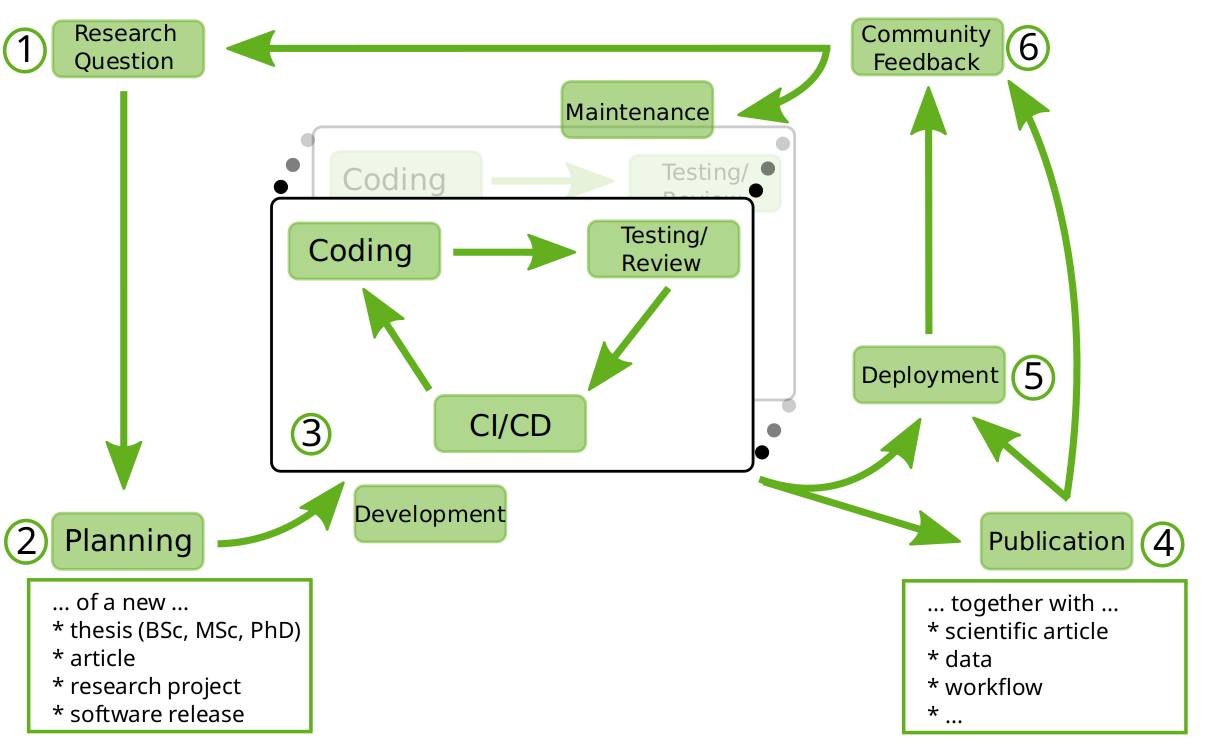
\includegraphics[width=0.85\linewidth]{imgs/rs_lifecycle.png}
    \caption{Research Software lifecycle. From \textit{sub-group 1} \cite{sg1tf2023}.}
    \label{fig:rslifecycle}
\end{figure}

\subsection{Document organization}

The structure of the document is as follows:

\begin{itemize}
    \item Section~\ref{sec:classification} describes a survey conducted within the sub-group. The objective was to search for articles and documents describing Quality Models and corresponding Quality Attributes or Quality Characteristics. The complete list of Quality Attributes are given in Appendix~\ref{appendix_qa}.
    
    \item In Section~\ref{sec:landscaping}, the RS stacks, RS types and user stories, are identified. This classification is important for the recommendations in next section.

    \item In Section~\ref{sec:recommendations}, recommendations are given for what Software Quality Attributes are more relevant for RS, depending on the stack, type and users or teams in their role as developers. There are also recommendations for software release and management and for services/platforms in production.
    
    \item In Section~\ref{sec:perspectives}, the user perspectives are described, i.e., the point of view of developers, users and resource (or service) providers.
    
    \item Section~\ref{sec:metadata} associates Quality Attributes and FAIR principles for RS.
    
    \item Last, the summary and conclusions are drawn in Section~\ref{sec:summary}.
\end{itemize}